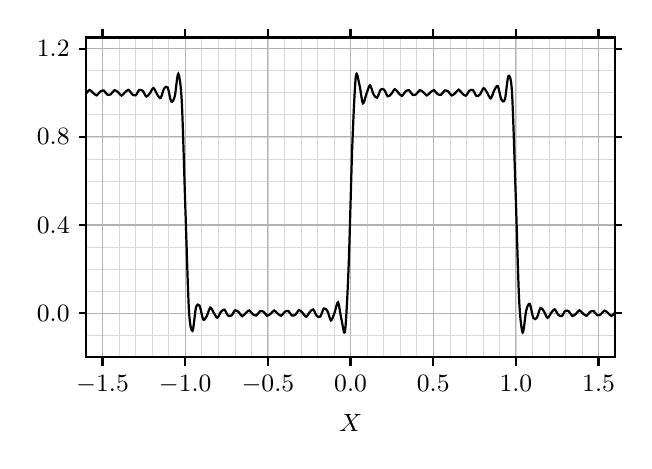
\begin{tikzpicture}[x=2.1cm, y=2.8cm]
        % Background Grid
        \draw[gray!30, line width=0.2pt, step=0.1] (-1.6,-0.2) grid (1.6,1.25);
        \draw[gray!60, line width=0.4pt, xstep=0.5, ystep=0.4] (-1.6,-0.2) grid (1.6,1.25);

        % Outer Bounding Box
        \draw[thick] (-1.6,-0.2) rectangle (1.6,1.25);

        % X-Axis Ticks & Labels
        \foreach \x in {-1.5, -1.0, -0.5, 0.0, 0.5, 1.0, 1.5} {
            \draw[thick] (\x,-0.2) -- (\x,-0.24);
            \draw[thick] (\x,1.25) -- (\x,1.29);
            \node[below, font=\small] at (\x,-0.24) {\pgfmathprintnumber[fixed,precision=1,zerofill]{\x}};
        }

        % Y-Axis Ticks & Labels
        \foreach \y in {0.0, 0.4, 0.8, 1.2} {
            \draw[thick] (-1.6,\y) -- (-1.64,\y);
            \draw[thick] (1.6,\y) -- (1.64,\y);
            \node[left, font=\small] at (-1.64,\y) {\pgfmathprintnumber[fixed,precision=1,zerofill]{\y}};
        }

        % Axis Label
        \node[below=14pt, font=\small] at (0,-0.24) {$X$};

        % Fourier Square Wave Plot
        \draw[thick, black, declare function={
            f(\x) = 0.5 + (2/pi)*(
                sin(deg(pi*\x)) 
                + (1/3)*sin(deg(3*pi*\x)) 
                + (1/5)*sin(deg(5*pi*\x)) 
                + (1/7)*sin(deg(7*pi*\x)) 
                + (1/9)*sin(deg(9*pi*\x)) 
                + (1/11)*sin(deg(11*pi*\x)) 
                + (1/13)*sin(deg(13*pi*\x)) 
                + (1/15)*sin(deg(15*pi*\x)) 
                + (1/17)*sin(deg(17*pi*\x)) 
                + (1/19)*sin(deg(19*pi*\x)) 
                + (1/21)*sin(deg(21*pi*\x)) 
                + (1/23)*sin(deg(23*pi*\x)) 
                + (1/25)*sin(deg(25*pi*\x))
            );
        }] 
        plot[domain=-1.6:1.6, samples=150, smooth] (\x, {f(\x)});
    \end{tikzpicture}

